\section{Theorie}
\label{sec:Theorie}

\subsection{Aufbau der Franck--Hertz-Apparatur}

Die für die Anregung nötige Energie wird von beschleunigten Elektronen aufgebracht, die mit den Hg-Atomen zusammenstoßen. 
Bei einem elastischen Stoßen werden die Elektronen durch ihre sehr viel geringere Masse nahezu reflektiert, ohne die Bewegung der 
schwereren Atome zu beeinflussen; bei einem inelastischen Stoß nehmen die Atome Energie auf und wechseln in einen angeregten Zustand.
Die reflektierten Elektronen sind in dem Fall entsprechend langsamer und haben weniger kinetische Energie. Durch Emission elektromagnetischer Wellen 
gehen die Hg-Atome anschließend wieder in ihren Grundzustand über. \cite{Versuchsanleitung}

Da die Energieniveaus gemäß der Theorie diskret sind, wird erwartet, dass bei einer Energie, die der Differenz zwischen 
zwei Energieniveaus entspricht, sehr viel mehr Elektronen kinetische Energie verlieren, also inelastisch mit den Atomen zusammenstoßen. 

\begin{figure}
    \centering
    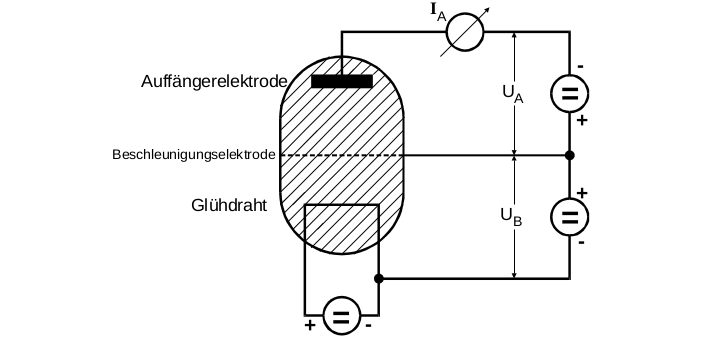
\includegraphics[width=\textwidth]{plots/schemaAufbau.png}
    \caption{Schematischer Aufbau der Franck--Hertz-Röhre\cite{Versuchsanleitung}.}
    \label{fig:schemaAufbau}
\end{figure}

Von der in Abbildung \ref{fig:schemaAufbau} gezeigten Apparatur wird erwartet, dass sie dies ausnutzen kann. 

Zu sehen ist eine evakuierte Röhre, in der sich ein winziger Tropfen Hg-Gas befindet. 
Der Druck kann mittels eines Temperaturreglers verändert werden, vergleiche dazu Abschnitt \ref{sub:Druck}. 
Am unteren Ende befindet sich der Glühdraht, an den eine vergleichsweise hohe Spannung angelegt wird. 
Diese soll so hoch sein, dass sie die Austrittsarbeit des Drahts, die für gewöhnlich möglichst niedrig gewählt ist, 
für Elektronen übersteigt, sodass Elektronen in der Lage sind, aus dem Draht auszutreten. 
Um die Austrittsarbeit weiter zu verringern, wird das hochschmelzende Metall (zum Beispiel Wolfram) zusätzlich mit 
einem Oxid eines Erdalkalimetalls beschichtet, dessen Austrittsarbeit sehr klein ist\cite{Versuchsanleitung}. 

Eine weitere angelegte Spannung ist die Beschleunigungsspannung $U_\text{B}$. 
Die positiv geladene Beschleunigunsanode soll die Elektronen in ihre Richtung beschleunigen.
Nach Durchlaufen des elektrischen Felds haben sie somit eine Energie von 
\begin{equation*}
    E=\symup{e}U_\text{B}
\end{equation*}
aufgenommen, wobei $\symup{e}=\SI{1.6021766208e-19}{\coulomb}$ die Elementarladung ist\cite{scipy}. 
Der negative Pol der Beschleunigungsspannung wird oft an einen kleinen, um den Glühdraht befindlichen Zylinder angeschlossen. 
Er hat eine Öffnung Richtung der Beschleunigunselektrode und dient dazu, die austretende Elektronenwolke durch ihre 
Coulomb-Abstoßung zu fokussieren.

Nach dem Erreichen der Beschleunigunselektrode haben die Elektronen also eine gewisse Energie, die je nach gewählter Spannung $U_\text{B}$
ausreicht, die Hg-Atome bei Stößen anzuregen beziehungsweise sogar zu ionisieren. Dadurch verlieren die Elektronen 
genau den Betrag der Energiedifferenz $\Delta E=E_1-E_0$.

Zur Auswertung der Elektronenenergie wird die Gegenfeldmethode benutzt. 

Wird ein zweites, dem ersten Feld entgegengesetztes elektrisches Feld mit der Bremsspannung $U_\text{A}$ angelegt, müssen die 
Elektronen zum Erreichen der Auffängerelektrode einen Teil ihrer Energie aufwenden. 
Je nachdem wie viele Elektronen also die Auffängerelektrode erreichen, kann eine Aussage darüber gemacht werden, 
wie viele Elektronen Energie durch inelastische Stöße mit den Hg-Atomen verlieren. 
Ein Maß für die Anzahl der ankommenden Elektronen wird durch den Auffängerstrom $I_\text{A}$ gegeben, der mithilfe eines 
Amperemeters hinter der Auffängerelektrode gemessen wird. 

Gemäß den vorangehenden Überlegungen wird in etwa eine Kurve erwartet, wie sie in Abbildung \ref{fig:erwartKurve} zu sehen ist. 
\begin{figure}
    \centering
    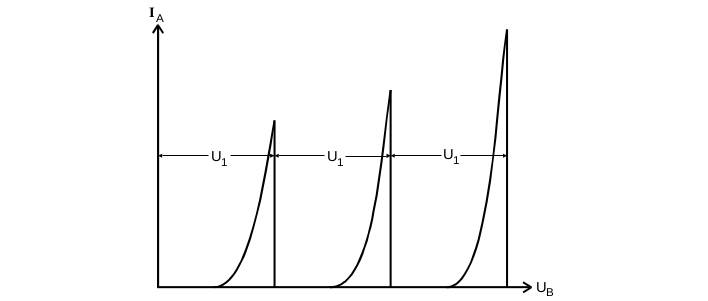
\includegraphics[width=\textwidth]{plots/erwartKurve.png}
    \caption{Theoretisch zu erwartende, ideale Kurve des Auffängerstroms in Abhängigkeit von der Beschleunigungsspannung\cite{Versuchsanleitung}.}
    \label{fig:erwartKurve}
\end{figure}
Immer dann, wenn die durch die Beschleunigungsspannung erhaltene kinetische Energie ausreicht, die Hg-Atome anzuregen, 
verlieren die beschleunigten Elektronen beim Durchlaufen der elektrischen Felder eine bestimmte, diskrete Energiedifferenz, 
wodurch auf einmal viel weniger Elektronen die Auffängerelektrode erreichen, weil deren Energie nicht mehr ausreicht, das 
zweite elektrische Feld zu durchlaufen. 
Es ist mehr als ein deutlicher Abfall des Auffängerstroms zu beobachten, da bei ausreichend großer Energie 
mehrere inelastischen Stöße ausgeführt werden können. 
Die Peaks befinden sich idealerweise in äquidistanten 
Abständen zueinander, deren Spannungsdifferenz gerade $\Delta E$ der Hg-Atome entpsricht, also\cite{Versuchsanleitung} 
\begin{equation*}
    U_1= \frac{1}{\symup{e}}\cdot (E_1-E_0)\:.
\end{equation*}

\subsection{Das Kontaktpotential}

Da der Glühdraht, aus dem die Elektronen austreten, eine von der Auffängerelektrode, von der die Elektronen wieder 
absorbiert werden, verschiedene Austrittsarbeit hat, sofern diese aus unterschiedlichen Materialien bestehen, ergibt 
sich eine Potentialdifferenz. Sie muss von dem dazwischen liegenden Potential abgezogen werden, um das tatsächliche 
Beschleunigungspotential zu ermitteln. 
Veranschaulicht wird dies in Abbildung \ref{fig:Kontaktpotential}.
\begin{figure}
    \centering
    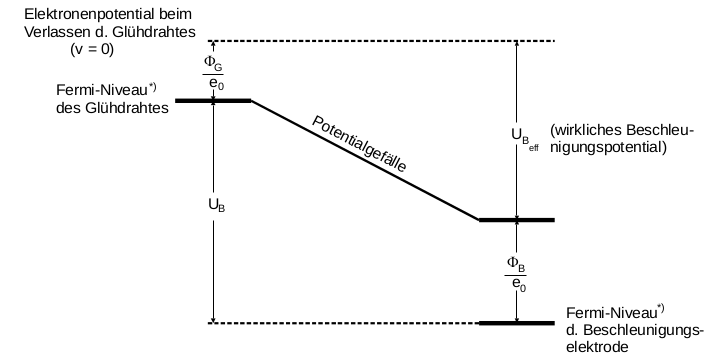
\includegraphics[width=\textwidth]{plots/Kontaktpotential.png}
    \caption{Schematische Darstellung zum Kontaktpotential\cite{Versuchsanleitung}.}
    \label{fig:Kontaktpotential}
\end{figure}
Aus diesen Überlegungen ergibt sich 
\begin{equation*}
    U_\text{B}+\frac{\phi_\text{G}}{\symup{e}} -U_\text{B,eff}+\frac{\phi_\text{B}}{\symup{e}}=0
\end{equation*}
\begin{equation*}
    \Leftrightarrow U_\text{B,eff}=U_\text{B}-K
\end{equation*}
\begin{equation*}
    \text{mit dem Kontaktpotential} \quad K:=\frac{1}{\symup{e}}\cdot (\phi_\text{B}-\phi_\text{G})\:.
\end{equation*}
Die Franck--Hertz-Kurve ist entsprechend um den Wert $K$ verschoben\cite{Versuchsanleitung}. 

\subsection{Energieverteilung der Elektronen}

Die Elektronen haben beim Austritt aus dem Glühdraht keine identische Energie, sondern haben ein durch die Fermi--Dirac-Statistik 
beschriebenes Energiespektrum. 
Dadurch können höherenergetische Elektronen bei einer geringeren Beschleunigungsspannung inelastische Stöße ausführen, 
wohingegen niederenergetische Elektronen nur elastisch stoßen. Dies führt dazu, dass die in Abbildung \ref{fig:erwartKurve}
ideal dargestellte Kurve abflacht und der Auffängerstrom ebenfalls nach Erreichen eines Maximums nicht ganz auf Null abfällt. 

Ebenfalls führen elastische Stöße im Bremsfeld dazu, dass sich die Geschwindigkeitskomponente in Richtung der Auffängerelektrode
verändert, auch wenn sich an der kinetischen Energie an sich nichts ändert. 
Da die besagte Geschwindigkeitskomponente jedoch für das Messen eines Auffängerstroms ausschlaggebend ist, folgt aus elastischen
Stößen ebenfalls ein Abflachen und Verbreitern der Kurve\cite{Versuchsanleitung}. 

\subsection{Regulierung des Dampfdrucks}
\label{sub:Druck}

Mithilfe der Temperatur des Hg-Gases wird der Druck reguliert, der wiederum die mittlere freie Weglänge beeinflusst. 
Die mittlere freie Weglänge muss so gewählt sein, dass eine hinreichend große Wahrscheinlichkeit besteht, dass die Elektronen 
mit den Hg-Atomen zusammenstoßen; gleichzeitig ist wichtig, dass nicht zu viele Stöße stattfinden, da sonst  
zu viele elastische Stöße stattfinden würden, die wie erwähnt die Kurve abflachen und verfälschen. 

Die mittlere freie Weglänge $\bar{w}$ ist antiproportional zum Druck $p$ gemäß 
\begin{equation}
    \bar{w}=\frac{\SI{2.9e-3}{\centi\meter}}{\frac{p}{\si{\milli\bar}}}\:;
    \label{eqn:Weglänge}
\end{equation}
der Druck ist wiederum mit der Temperatur über 
\begin{equation*}
    p(T)=\SI{5.5e7}{\milli\bar}\cdot \symup{e}^{\frac{\SI{-6876}{\kelvin}}{T}}
\end{equation*}
verknüpft. 
Ein idealer Dampfdruck für die verwendete Apparatur ergibt eine mittlere freie Weglänge, die um einen Faktor von etwa 
$1000$ bis $4000$ kleiner ist als der Abstand zwischen Beschleunigunsanode und Glühkathode $a\approx \SI{1}{\centi\meter}$. 
Daraus lässt sich die Temperatur ableiten, auf die die evakuierte Röhre geregelt werden muss\cite{Versuchsanleitung}. 

\subsection{Das Energieschema des Quecksilberatoms}

Das Quecksilberatom ist bis zur 5p-Unterschale mit 54 Elektronen gemäß des Aufbauprinzips vollständig gefüllt; 
die 4f-Schale enthält weitere 14 Elektronen, die 5d-Schale 10 Elektronen und zwei Elektronen befinden sich in der 6s-Schale. 
Somit besitzt das Atom insgesamt 80 Elektronen im ungeladenen Zustand. 

Die Elektronen in der 6s-Schale befinden sich in dem antiparallelen Singulett-Zustand, sodass sie sich gemäß des Pauli-Prinzips 
in mindestens einer Quantenzahl unterscheiden. 
Zusätzlich muss die Auswahlregel für die Quantenzahl $L$ des Bahndrehimpulses beachtet werden. 
Die Differenz zum angeregten Zustand muss genau $\Delta L=\pm 1$ betragen. 

Für die Elektronen des nicht-angeregten Zustands mit den Quantenzahlen 
\begin{equation*}
    n_1=n_2=6\:,\quad l_1=l_2=0\:,\quad s_1=\frac{1}{2}\:,\quad s_2=\frac{-1}{2}
\end{equation*}
bedeutet dies, dass $l_1$ oder $l_2$ den Wert $1$ annehmen muss, wohingegen die jeweils andere Quantenzahl gleich bleibt. 
Im angeregten Zustand unterscheiden sich die beiden Elektronen also bereits in einer Quantenzahl, weshalb eine parallele Stellung 
hier möglich ist. 

\begin{figure}
    \centering
    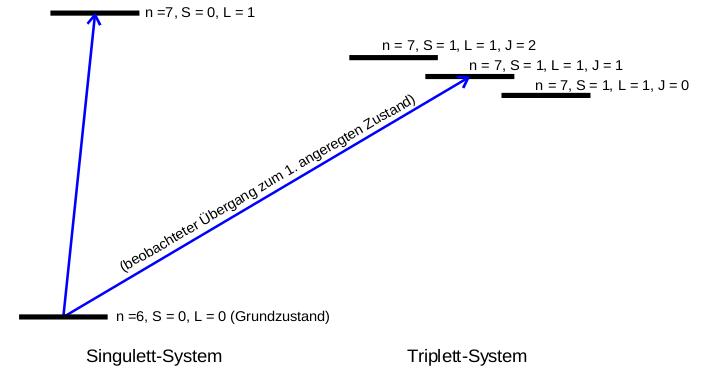
\includegraphics[width=\textwidth]{plots/Energieschema.png}
    \caption{Nicht-maßstabsgetreue Veranschaulichung des Energieschemas im Hg-Atom\cite{Versuchsanleitung}.}
    \label{fig:Energieschema}
\end{figure}

Die relative Lage der Spins zueinander beeinflusst, wie nah sich die Elektronen zueinander befinden. Bei antiparalleler Stellung 
sind sie näher zusammen, als wenn sie parallel zueinander sind. 
Da bei einem geringeren Abstand die Energie durch die Coulomb-Abstoßung steigt, ist der Triplett-Zustand (parallel) energetisch 
günstiger als der Singulett-Zustand (antiparallel).
Dementsprechend wird in diesem Experiment vor allem der Übergang in den Triplett-Zustand beobachtet. 

Diese Energie ist durch die LS-Kopplung dreifach entartet, hier kann also eine Feinstruktur im Gegensatz zum Grundzustand beobachtet werden. 

Ein Umklappen eines Spins (wie es hier nötig ist, schließlich gehen die Elektronenspins von einem antiparallelen in einen 
parallelen Zustand über) ist vergleichsweise sehr unwahrscheinlich, was durch das Interkombinationsverbot beschrieben wird. 
Da in diesem Experiment jedoch Elektronenstöße zur Anregung verwendet werden, wird dieses Problem dadurch umgangen, dass 
das stoßende Elektron den Platz eines Elektrons mit genau entgegengerichtetem Spin einnimmt und das herausgelöste Elektron mit 
der entsprechenden Restenergie weiterpropagiert. 

Das Energieschema der beiden für die Anregung wichtigen Elektronen wird in Abbildung \ref{fig:Energieschema} veranschaulicht\cite{Versuchsanleitung}. 
